\documentclass{article}

\usepackage[utf8]{inputenc}
\usepackage{array}

\usepackage{amsmath}
\usepackage{amssymb}

\usepackage{graphicx}
\usepackage{tabularx}
\usepackage[letterpaper, total={6.5in, 9in}]{geometry}

\usepackage{multirow}

\usepackage{url}

\graphicspath{ {Images/} }
% !TeX spellcheck = en_GB


\begin{document}

\title{A Geometric Explanation for Prime-rich Lines on the Ulam Spiral}
\author{Justin Xu}
\date{3 January 2019}
\pagenumbering{gobble}

\maketitle
\begin{center}
	\textbf{Mathematics} \\
	\textit{How can a model based on the cause of prime-rich lines in the Ulam spiral be used to produce prime numbers?} \\
	3982 words
\end{center}

\newpage
\tableofcontents

\newpage
\pagenumbering{arabic}



\section{Introduction}

On the Cartesian plane, the natural numbers are uniquely assigned to all points of integer coordinates (the lattice points) \((x,y)\). The mapping goes: \((0, 0) \mapsto 1\), \((1, 0) \mapsto 2\), \((1, 1) \mapsto 3\), \((0, 1) \mapsto 4\), \((-1, 1) \mapsto 5\), \((-1, 0) \mapsto 6\), \((-1, -1) \mapsto 7\), \((0, -1) \mapsto 8\), \((1, -1) \mapsto 9\), \((2, -1) \mapsto 10\), \((2, 0) \mapsto 11\), \((2, 1) \mapsto 12\), \((2, 2) \mapsto 13\), and continues infinitely outward, as described by Stanislaw Ulam (after whom the spiral is named), Myron Stein, and Mark Wells in \textit{A Visual Display of Some Properties of the Distribution of Primes}. In Figure \ref{fig:f}, connecting points that have been assigned consecutive numbers results in a counterclockwise square spiral---the Ulam spiral.

\begin{figure}[h!]
	\centering
	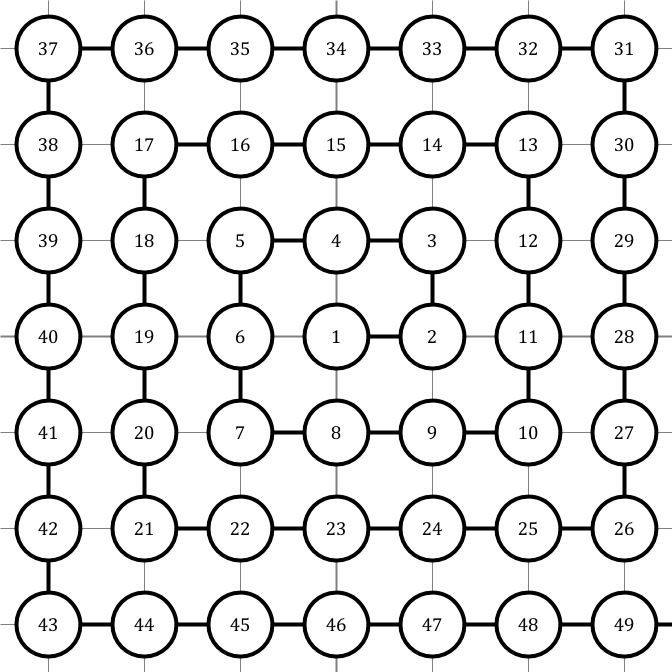
\includegraphics[scale=0.6]{f}
	\caption{Lattice points in the domain \(|x|,|y|{\leq}3\) are shown as circles containing the number assigned to them.}
	\label{fig:f}
\end{figure}

In the most common image of the spiral, each lattice point is represented as a single pixel. ``Prime points'' have been assigned prime numbers, and are coloured black. The curiosity of the spiral is the presence of prominent ``prime-rich lines'', along which prime points occur with a greater-than-expected frequency. The existence of prime-rich lines is surprising to some, because it shows a pattern that is not intuitively expected. For this reason, the Ulam spiral is popularized as mysterious.

\begin{figure}[h!]
	\centering
	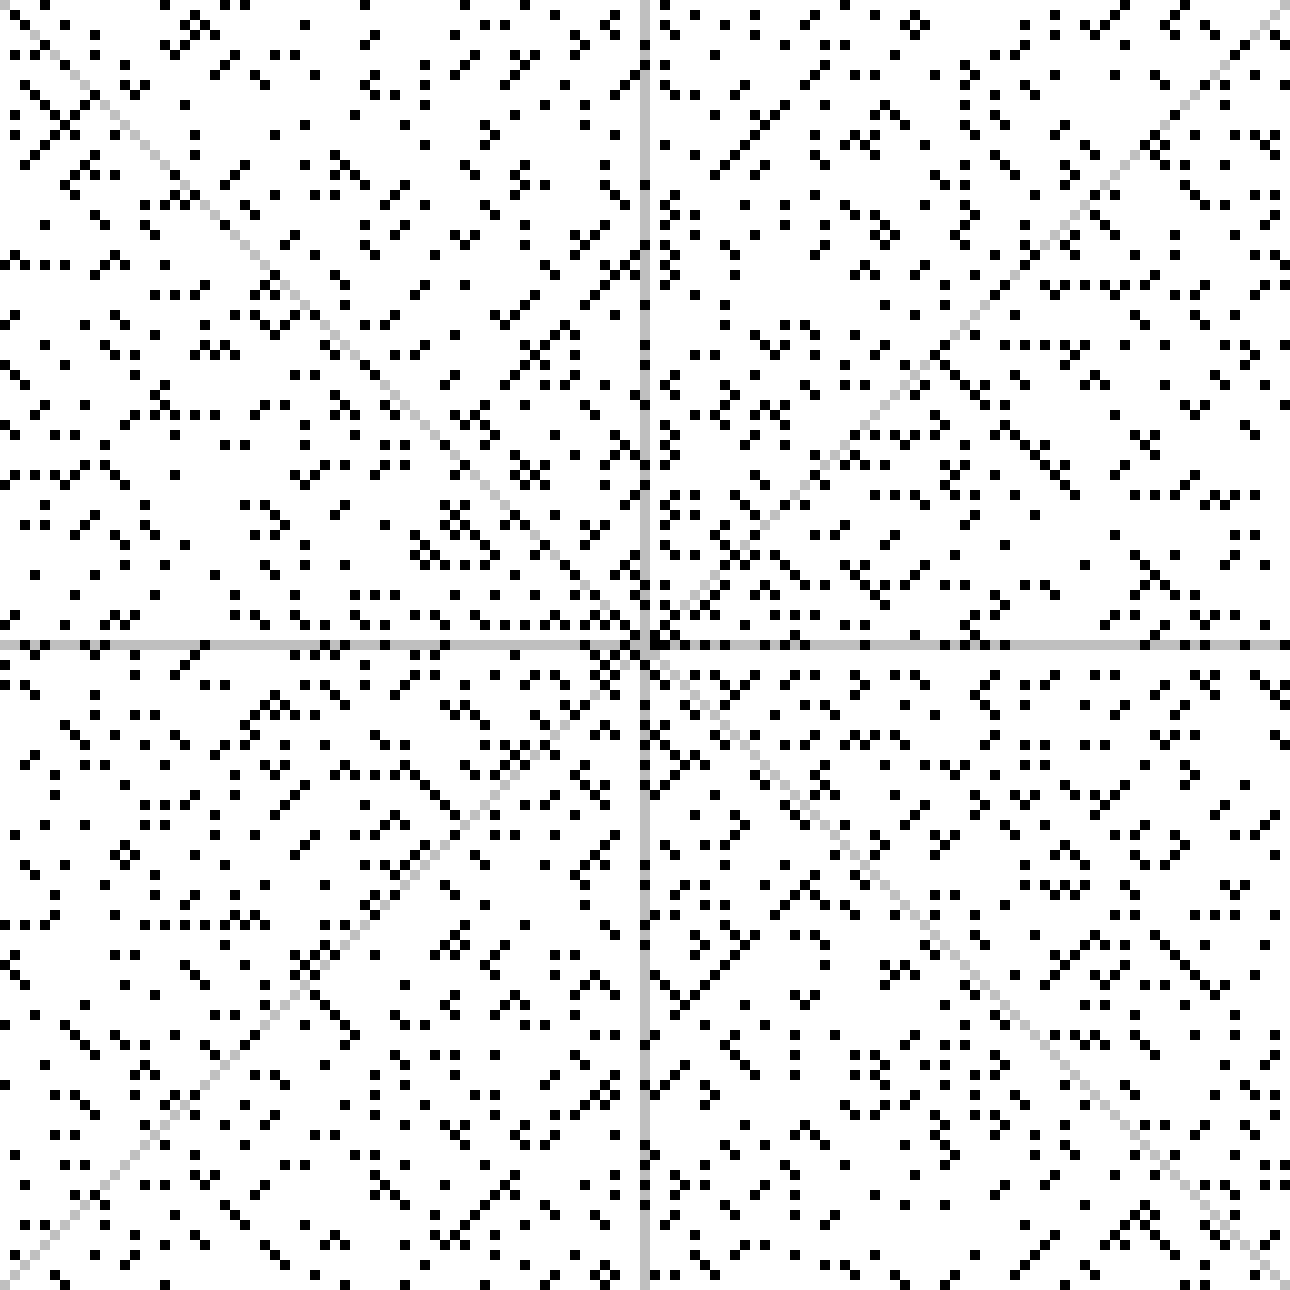
\includegraphics[width=\textwidth]{ulamspiral}
	\caption{Points \(|x|,|y|\leq64\) in the Ulam spiral, coloured as described. Lines \(x=0\), \(y=0\), and \(y=\pm x\) are also shown.}
	\label{ulamspiral}
\end{figure}

In the original paper, prime-rich lines are stated to be connected to the factorability of quadratic expressions. Robert Sacks thoroughly explains this connection using a round (Archimedean) variant of the spiral. Nonetheless, understanding of the Ulam spiral is incomplete. It receives little attention, the majority of which is from amateur mathematicians. This essay presents an in-depth study of an incomplete explanation first mentioned by Tom Bates. It focuses on geometric patterns that appear when points assigned values divisible by a particular number are highlighted. The explanation is implemented in a model to predict the locations of prime points in the spiral. The success of this model leads reflects the success of the explanation, leading to the question: \textit{How can a model based on the cause of prime-rich lines in the Ulam spiral be used to produce prime numbers?}



\section{Modelling the spiral}

\subsection{Wheel factorization}

For a factor \(p\), the probability that a randomly chosen number \(X\) is indivisible by \(p\) is \(\frac{p-1}{p}\). \(X\) is prime (\(X \in \mathbb{P}\)) if it is indivisible by every prime number between \(2\) and \(\sqrt{X}\) (inclusive). Suppose \(X\) has a value close to \(x\). Then, probabilistic arguments can be made:
	\[P(X \in \mathbb{P}|X \approx x) \approx P((p_1 \nmid X)\cap(p_2 \nmid X)\cap\ldots\cap(p_k \nmid X))\]

Where \(p_n\) is the \(n\)th prime, and \(k\) is the number of primes less than \(\sqrt{x}\). Each event \(p \nmid X\) is independent:
\begin{align}
	\nonumber \therefore P(X \in \mathbb{P}|X \approx x) &\approx P(p_1 \nmid X)\times P(p_2 \nmid X)\times\ldots\times P(p_k \nmid X) \\
	\nonumber \therefore P(X \in \mathbb{P}|X \approx x) &\approx \frac{p_1-1}{p_1}\times \frac{p_2-1}{p_2}\times\ldots\times \frac{p_k-1}{p_k}=\prod_{i=1}^{k}\frac{p_i-1}{p_i} \approx \frac{1}{\ln(x) - 1.08366}
\end{align}

Then, one is given that \(X\) is not a multiple of \(p_n\), where \(1 \leq n \leq k\).
\begin{align}
	\nonumber P(X \in \mathbb{P}|X \approx x,p_n \nmid X) &= \frac{P(X \in \mathbb{P}|X \approx x)\cap (p_n \nmid X))}{P(p_n \nmid X)} = \frac{P(X \in \mathbb{P}|X \approx x)}{\frac{p_n-1}{p_n}} \\
	\nonumber P(X \in \mathbb{P}|X \approx x,p_n \nmid X) &= \frac{p_n}{p_n-1}P(X \in \mathbb{P}|X \approx x)
\end{align}

Such given information is desirable, as it increases the probability of finding a prime number when \(X\) is chosen. Let \(Q\) represent the factor by which \(P(X \in \mathbb{P}|X \approx x)\) increases. Then, the probability that \(X\) is prime is approximately \(\frac{Q}{\ln(x) - 1.08366}\). In the above case, \(Q=\frac{p_n}{p_n-1}\). Ideally, \(Q\) should be as large as possible. Wheels use multiple conditions to result in large values of \(Q\):

\begin{enumerate}
	\item \(2 \nmid X \iff X \not\equiv 0\ (\text{mod }2)\).
	\item \(3 \nmid X \iff X \not\equiv 0\ (\text{mod }3)\).
	\item The Chinese remainder theorem states that the conditions can be combined to find \(X\) modulo \(2 \times 3 = 6\). Assume \(X\) can be congruent to anything modulo 6: \(X \equiv 0,1,2,3,4,5\ (\text{mod }6)\).
	\item \(X \not\equiv 0\ (\text{mod }2)\), \(\therefore X \equiv 1,3,5\ (\text{mod }6)\).
	\item \(X \not\equiv 0\ (\text{mod }3)\), \(\therefore X \equiv 1,5\ (\text{mod }6)\).
\end{enumerate}
	
\(X \equiv 1,5\ (\text{mod }6)\) is an example of a wheel. Selecting \(X\) to equal \(1+6k\) or \(5+6k\) introduces some information about \(X\), such that \(Q=\frac{2}{2-1}\frac{3}{3-1}=3\). Adding more statements like \(5 \nmid p\) can increase \(Q\) further. Similarly on the Ulam spiral, a more complicated process may locate lines that contain no points that have been assigned multiples of the first \(n\) primes---the prime-rich lines.


\subsection{Goals of a model}

The primary goal of the model presented in this essay is to predict the locations of prime-rich lines in the Ulam spiral. This is evaluated based on how prime-rich these lines are, compared to a random selection of ``average'' lines. The greater the difference, the more effectively the model may be used to produce primes. The exploration is also driven by the goal to be as complete as possible in describing the mechanics of the spiral. Many amateur studies are incomplete due to a limited focus, such as on lines of a particular slope. This essay attempts to avoid specific cases as much as possible. Finally, computational complexity is an important theme in the development of algorithms used to find prime numbers. In this exploration, symmetries are studied as a means to minimize computation.

Along with the model, most images of the spiral that appear in this essay are generated with the assistance of original Java code, which may be found in the appendix.



\section{Spiral anatomy}

\subsection{The spiral as a recursive function}

\(f\) is a function accepting a lattice point (\((x,y) \in \mathbb{Z}\times\mathbb{Z}\)) as its parameter, that outputs the number assigned to that point on the Ulam spiral. The recursive definition of \(f\) is similar to the way in which a person might construct the spiral.
	\[f((x,y)) = \begin{cases}
				 1,				&\text{if } (x,y) = (0,0) \\
				 f((x,y-1))+1,	&\text{if } -x+2 \leq y \leq x		\hfill \quad \text{in quadrant } 1\\
				 f((x+1,y))+1,	&\text{if } -y\leq x \leq y-1		\hfill \quad \text{in quadrant } 2\\
				 f((x,y+1))+1,	&\text{if } x \leq y \leq -x-1		\hfill \quad \text{in quadrant } 3\\
				 f((x-1,y))+1,	&\text{if } y+1 \leq x \leq -y+1	\hfill \quad \text{in quadrant } 4
				 \end{cases}\]

Four quadrants exist on the spiral. In each quadrant ``the next point'' is in a different direction relative to the previous point. The variable \(d\) represents the quadrant number, an arbitrary value from 1 to 4. In this essay, \(d=D\) is used to signify that only quadrant \(D\) is being considered.
	\[d = \begin{cases}
		  1,	&\text{if } -x+2 \leq y \leq x\\
		  2,	&\text{if } -y \leq x \leq y-1\\
		  3,	&\text{if } x \leq y \leq -x-1\\
		  4,	&\text{if } y+1 \leq x \leq -y+1
		  \end{cases}\]

In all quadrants, some unit vector describes the displacement to a point from ``the point before it''. Let \(\hat{v}\) represent this vector:
	\[\hat{v} = (v_x,v_y) = \begin{cases} 
							(0,1),	&\text{if }d=1\\
							(-1,0),	&\text{if }d=2\\
							(0,-1),	&\text{if }d=3\\
							(1,0),	&\text{if }d=4\\
							\end{cases}\]
							
By definition, \(f\) can be rewritten as:
	\[f((x,y)) = \begin{cases}
				 1,						&\text{if } (x,y) = (0,0) \\
				 f((x,y)-\hat{v}) + 1, 	& \text{otherwise} \\
				 \end{cases}\]

The spiral winds around the origin by one ``layer'' per complete revolution. A separate vector \(\hat{u}\) represents the direction between successive layers of the spiral. For example, \((6,2)\) is one layer beyond \((5,2)\) in quadrant 1.
	\[\hat{u} = (u_x,u_y) = \begin{cases}
							(1,0),	&\text{if }d=1\\
							(0,1),	&\text{if }d=2\\
							(-1,0),	&\text{if }d=3\\
							(0,-1),	&\text{if }d=4\\
							\end{cases}\]

\(a\hat{u}+b\hat{v}\) is a frequent representation of points in this essay. \(a\) is the number of layers between the point and the origin, and \(b\) represents how far anticlockwise the point is in the rotation of the spiral. \(a\) and \(b\) must be integers. When writing \(a\hat{u}+b\hat{v}\), the location of the point is ambiguous, since the unit vectors depend on the undeclared quadrant number \(d\). Writing \(d=D:a\hat{u}+b\hat{v}\), there is no ambiguity, since the unit vectors are defined. Every point has a unique representation in the form \(d=D:a\hat{u}+b\hat{v}\).
				 
\begin{figure}[h!]
	\centering
	\begin{tabular}{cc}
		
\includegraphics[width=0.4\textwidth]{quadrants} & 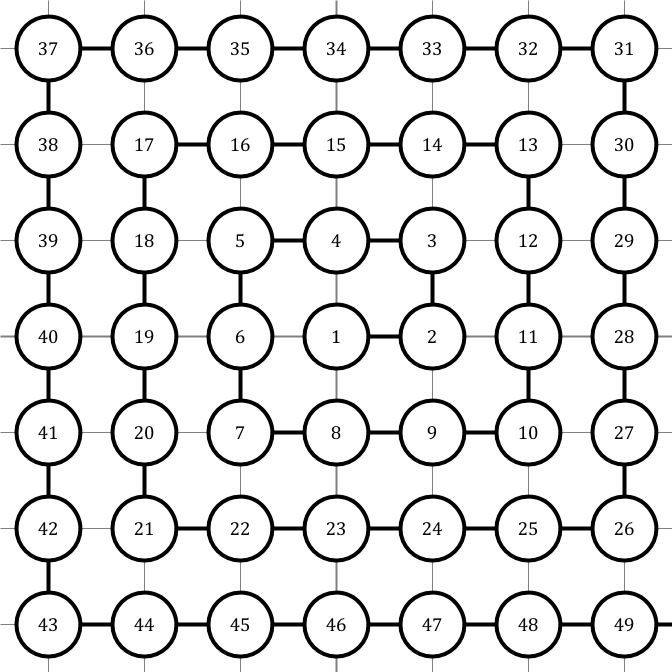
\includegraphics[width=0.4\textwidth]{f}
	\end{tabular}
	\caption{The quadrants: 1) red, 2) yellow, 3) green, 4) blue. Black arrows represent \(\hat{u}\), white arrows represent \(\hat{v}\). The point assigned 14 is located at \(d=2:2\hat{u}+(-1)\hat{v}\). In comparison, \(d=3:f(2\hat{u}+(-1)\hat{v})=18\).}
	\label{quadrants}
\end{figure}

%By selecting a value for \(d\), one defines \(\hat{u}\) and \(\hat{v}\), as well as selecting a quadrant where the point \(a\hat{u}+b\hat{v}\) is expected to be. The point can be outside the quadrant, in which case it is treated as invalid and ignored. A representation such as \(-2\hat{u}+1\hat{v}\) is never valid, no matter which value is chosen for \(d\). For valid points \(a\) is never negative, just as it makes no sense for there to be a negative layer on a spiral.

\paragraph{The generalized spiral} The Ulam spiral can be generalized to begin with \(n\) at \((0,0)\) and increment by \(m\).
	\[f_{m,n}((x,y)) = \begin{cases}
					   n,							&\text{if } (x,y) = (0,0) \\
					   f_{m,n}((x,y)-\hat{v}) + m,	& \text{otherwise} \\
					   \end{cases}\]
						 
The original Ulam spiral is described by \(f_{1,1}\). This complication is not solely for being general. The range of \(f\) can be set to any arbitrary arithmetic sequence: \(f_{m,n}(P) \equiv n\ (\text{mod }m)\). Thus, wheel factorization may be directly implemented into the Ulam spiral. For example, the wheel \(p \equiv 1,5\ (\text{mod }m)\) can be simulated with \(f_{6,1}\) and \(f_{6,5}\).


\subsection{The spiral as an explicit function}

Performing recursion is computationally intensive; an explicit function is more desirable. Examining the relationship between \(a\) and \(f_{m,n}(a\hat{u}))\), quadratic relationships are found.

\begin{center}
	\begin{tabular}{|c|c|c|c|c|}
		\hline
		\(a\) & \(d=1\) & \(d=2\) & \(d=3\) & \(d=4\) \\
		\hline
		1 & \(1m+n\) & \(3m+n\) & \(5m+n\) & \(7m+n\) \\
		\hline
		2 & \(10m+n\) & \(14m+n\) & \(18m+n\) & \(22m+n\) \\
		\hline
		3 & \(27m+n\) & \(33m+n\) & \(39m+n\) & \(45m+n\) \\
		\hline
		4 & \(52m+n\) & \(60m+n\) & \(68m+n\) & \(76m+n\) \\
		\hline
		5 & \(85m+n\) & \(95m+n\) & \(105m+n\) & \(115m+n\) \\
		\hline
		General & \((4a^2-3a)m+n\) & \((4a^2-a)m+n\) & \((4a^2+a)m+n\) & \((4a^2+3a)m+n\) \\
		formula & \scriptsize{\((4a^2-5a+2(1)a)m+n\)} & \scriptsize{\((4a^2-5a+2(2)a)m+n\)} & \scriptsize{\((4a^2-5a+2(3)a)m+n\)} & \scriptsize{\((4a^2-5a+2(4)a)m+n\)} \\
		\hline
	\end{tabular}
\end{center}

It is concluded from inspection that \(f_{m,n}(a\hat{u}) = (4a^2-5a+2da)m + n\). This can be substituted into the recursive formula for the generalized Ulam spiral.
	\[f_{m,n}(a\hat{u}+b\hat{v}) = \begin{cases}
					   			   (4a^2-5a+2da)m+n,						&\text{if } b = 0 \\
								   f_{m,n}(a\hat{u}+b\hat{v}-\hat{v}) + m,	& \text{otherwise} \\
					   			   \end{cases}\]

Thus, \(f_{m,n}(a\hat{u}+1\hat{v})=(4a^2-5a+2da)m+m+n\), which then allows \(f_{m,n}(a\hat{u}+2\hat{v})\) to be defined, and so on. By inductive reasoning, the explicit function of the generalized Ulam spiral is obtained:
	\[f_{m,n}(a\hat{u}+b\hat{v})=(4a^2-5a+2da)m+bm+n=(4a^2-5a+2da+b)m+n\]
	


\section{Divisibility plots}

\begin{figure}[h!]
	\centering
	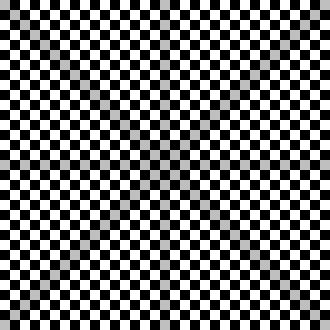
\includegraphics[scale=0.4]{div2}
	\caption{The plot of \(2 \mid f_{1,1}(P)\) shows why the prominent prime-rich lines on the Ulam spiral are primarily diagonal. Only a diagonal line may contain no multiples of 2.}
	\label{div2}
\end{figure}

The famous image of the Ulam spiral is a graph of \(f_{m,n}(P) \in \mathbb{P}\). This is not the only possible representation. In this section, the graph of \(p \mid f_{m,n}(P)\) is explored in depth, called a ``divisibility plot'' modulo \(p\). No specific value of \(p\) is chosen, but it is understood that \(p\) is some odd prime number, treated as a constant.

\begin{figure}[h!]
	\centering
	\begin{tabular}{ccc}
		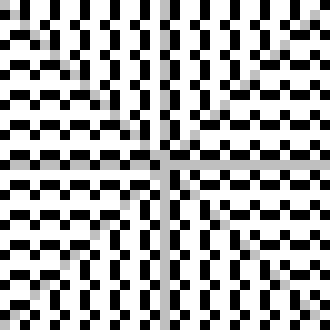
\includegraphics[scale=0.4]{div3} & 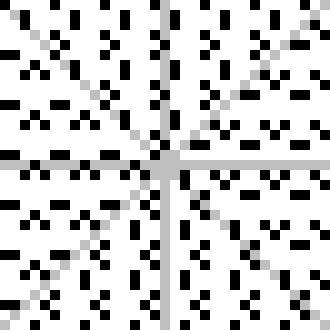
\includegraphics[scale=0.4]{div5} & 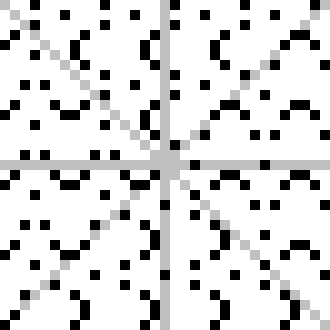
\includegraphics[scale=0.4]{div7} \\
		\(f_{1,1}(P) \equiv 0 \mod 3\) & \(f_{1,1}(P) \equiv 0 \mod 5\) & \(f_{1,1}(P) \equiv 0 \mod 7\) \\
	\end{tabular}
	\caption{Various divisibility plots.}
	\label{div}
\end{figure}


\subsection{Exceptions}

The mathematics presented in the following sections assume \(p \nmid m\). Recall that \(f_{m,n}(P) \equiv n\ (\text{mod }m)\). If \(p \mid m\), then \(f_{m,n}(P) \equiv n\ (\text{mod }p)\). If \(p \mid n\), then every point is divisible modulo \(p\), otherwise \(p \nmid n\) and no point is divisible.


\subsection{Parabolas}

Divisibility plots are named so because every point where \(p \mid f_{m,n}(P)\) is true has been assigned a multiple of \(p\). These points are ``divisible points''. If \(p \nmid f_{m,n}(P)\), \(P\) is an ``indivisible point''. Divisible points can be located explicitly:
\begin{align}
	\nonumber p \mid f_{m,n}(a\hat{u}+b\hat{v}) \iff f_{m,n}(a\hat{u}+b\hat{v}) \equiv (4a^2 - 5a + 2da + b)m + n &\equiv 0\ (\text{mod } p) \\
	\nonumber (4a^2 - 5a + 2da + b)m &\equiv -n\ (\text{mod } p) \\
	\nonumber 4a^2 - 5a + 2da + b &\equiv -m^{-1}_pn\ (\text{mod } p) \\
	\nonumber b &\equiv -4a^2 + 5a - 2da - m^{-1}_pn\ (\text{mod } p)
\end{align}
\[b = (-4+k_2p)a^2 + (5-2d+k_1p)a + (-m^{-1}_pn+k_0p),\ k_0,k_1,k_2 \in \mathbb{Z}\]
	
Thus, if \(a\hat{u}+b\hat{v}\) is a divisible point, then \(b\) is equal to a function \(g_{k_0,k_1,k_2}\) of \(a\):
	\[b = g_{k_0,k_1,k_2}(a) = (-4+k_2p)a^2 + (5-2d+k_1p)a + (-m^{-1}_pn+k_0p)\]

The notation \(m^{-1}_p\) is used throughout this essay to signify the least positive modular multiplicative inverse of \(m\) modulo \(p\). It is the solution to \(m^{-1}_pm \equiv 1\ (\text{mod } p)\ ,\ 0 \leq m^{-1}_p < p\). \(m^{-1}_p\) does not exist if \(m\) and \(p\) share a common factor. As \(k_0\), \(k_1\), \(k_2\), and \(a\) vary, every possible solution for \(b\) in \(f_{m,n}(a\hat{u}+b\hat{v}) \equiv 0\quad(\text{mod } p)\) is obtained. That is, \(a\hat{u}+g_{k_0,k_1,k_2}(a)\hat{v}\) describes every divisible point. Noting that \(g_{k_0,k_1,k_2}(a)\) is a quadratic expression, \(t\hat{u}+g_{k_0,k_1,k_2}(t)\hat{v}\ ,\ t \in \mathbb{Z}\) is a parabola consisting solely of divisible points. Varying \(k_0,k_1,k_2\) affects the behaviour of the parabola.

\begin{figure}[h!]
	\centering
	\begin{tabular}{ccc}
		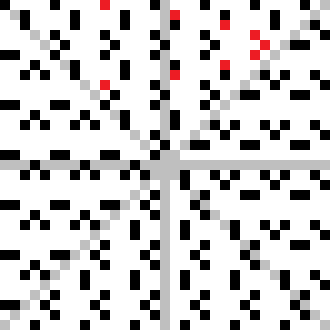
\includegraphics[scale=0.5]{m1_n1_p5_d} & 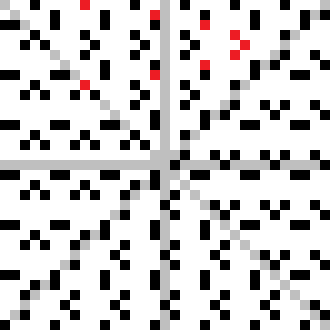
\includegraphics[scale=0.5]{m3_n7_p5_d} & 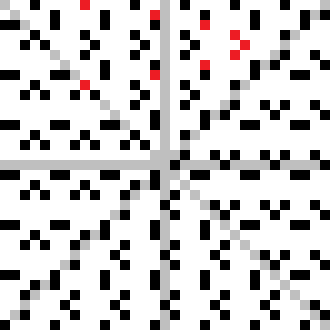
\includegraphics[scale=0.5]{m8_n2_p5_d} \\
		\(f_{1,1}\) & \(f_{3,7}\) & \(f_{8,2}\)
	\end{tabular}
	\caption{Various divisibility plots modulo 5. Example parabolas are highlighted in red.}
	\label{parabolas}
\end{figure}

\subsection{Symmetries}

Observations are made of three symmetries on the divisibility plot. They are transformations applied to a point, which guarantee that the transformed point is divisible, if the original is. The point resulting from the transformation is thus said to be ``redundant'' to the original. Redundancy is an equivalence relation on a divisibility plot:

\begin{itemize}
	\item Let \(A \rightleftharpoons B\) signify that \(B\) is divisible if \(A\) is. That is, \(B\) is redundant to \(A\). In terms of points, this means that a transformation following one of the three symmetries can move \(A\) to the location of \(B\).
	\item Reflexivity: \(A \rightleftharpoons A\).
	\item Symmetry: \(A \rightleftharpoons B \Rightarrow B \rightleftharpoons A\).
	\item Transitivity: \((A \rightleftharpoons B \land B \rightleftharpoons C) \Rightarrow A \rightleftharpoons C\).
\end{itemize}


\subsection{Translation symmetry}

\begin{figure}[h!]
	\centering
	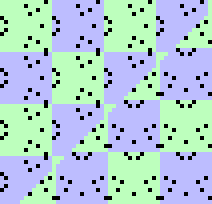
\includegraphics{tiling}
	\caption{The boundary between quadrants 1 and 2 in the divisibility plot modulo 13. In each quadrant, a pattern of divisible points repeats in both dimensions as tessellating \(13 \times 13\) square ``tiles''. This observation leads to the tiling conjecture.}
	\label{tiling}
\end{figure}

\paragraph{Tiling conjecture} \(P = a\hat{u}+b\hat{v}\) and \(P' = P + \Delta a\hat{u} + \Delta b\hat{v}\) are two points within the same quadrant. When \(\Delta a\) and \(\Delta b\) are multiples of \(p\), \(P'\) must be a divisible point if \(P\) is; \(P \rightleftharpoons P'\). Formally:
	\[P \rightleftharpoons P + k_ap\hat{u} + k_bp\hat{v}\ ,\ k_a,k_b \in \mathbb{Z}\]

\paragraph{Proof} Assume that \(P = a\hat{u}+b\hat{v}\) is a divisible point. That is,
	\[f_{m,n}(P) = f_{m,n}(a\hat{u}+b\hat{v}) = (4a^2 - 5a + 2da + b)m + n \equiv 0 \mod p\]
	
\(P'\) is a divisible point if \(f_{m,n}(P') \equiv 0 \mod p\).
	\[P' = P + \Delta a\hat{u} + \Delta b\hat{v} = (a + \Delta a)\hat{u} + (b + \Delta b)\hat{v}\]
	
When \(\Delta a\) and \(\Delta b\) are multiples of \(p\), they can be written as \(k_ap\) and \(k_bp\) respectively (\(k_a,k_b \in \mathbb{Z}\)).
\begin{align}
	\nonumber P' &= (a + k_ap)\hat{u} + (b + k_bp)\hat{v} \\
	\nonumber f_{m,n}(P') &= f_{m,n}((a + k_ap)\hat{u} + (b + k_bp)\hat{v}) \\
	\nonumber f_{m,n}(P') &= (4(a + k_ap)^2 - 5(a + k_ap) + 2d(a + k_ap) + (b + k_bp))m + n
\end{align}
\begin{align}
	\nonumber f_{m,n}(P') &= (4a^2 - 5a + 2da + b)m + (8ak_a + k_a^2p - 5k_a + 2dk_a + k_b)pm + n \\
	\nonumber f_{m,n}(P') &\equiv (4a^2 - 5a + 2da + b)m + n\ (\text{mod } p) \\
	\nonumber \text{It is known that }(4a^2 - 5a + 2da + b)m + n &\equiv 0\ (\text{mod } p) \\
	\nonumber \therefore f_{m,n}(P') &\equiv 0\ (\text{mod } p)
\end{align}

Therefore \(P'\) is a divisible point and the conjecture is proven.


\subsection{Reflection symmetry}

\begin{figure}[h!]
	\centering
	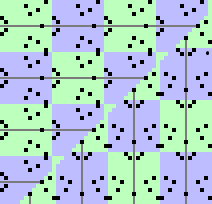
\includegraphics{reflection}
	\caption{The same plot from Figure \ref{tiling}, with lines of reflection drawn. The lines are parallel to \(\hat{v}\), separated by distances of \(p\). This observation leads to the reflection conjecture.}
	\label{reflection}
\end{figure}
	
\paragraph{Reflection conjecture} Lines of reflection can be described in vector form by \(A\hat{u}+t\hat{v}\ ,\ t \in \mathbb{Z}\), or \(a=A\). \(P = (A + \Delta a)\hat{u}+b\hat{v}\) and \(P' = A - \Delta a)\hat{u}+b\hat{v}\) are two points in the same quadrant. \(\Delta a\) is the distance from \(P\) and \(P'\) to \(a=A\). If \(P\) is a divisible point, then \(P'\) is as well.
	\[(A + \Delta a)\hat{u}+b\hat{v} \rightleftharpoons (A - \Delta a)\hat{u}+b\hat{v}\]

\paragraph{Proof} Every divisible point \(P\) is part of a parabola \(a\hat{u}+g_{k_0,k_1,k_2}(a)\hat{v}\). Every parabola has an axis of reflection symmetry; \(P\) can be reflected across this axis to the location \(P'\). Since \(P'\) is part of the parabola, it must be divisible. Thus, the axis of reflection of the parabola is the line of reflection described by the conjecture.

The axis of reflection of any parabola passes through its vertex, where the rate of change of \(g_{k_0,k_1,k_2}\) is zero:
\begin{align}
	\nonumber \therefore g'_{k_0,k_1,k_2}(A) = 2(-4 + k_2p)A + (5 - 2d + k_1p) &= 0 \\
	\nonumber -8A + 2k_2pA + 5 - 2d + k_1p &= 0 \\
	\nonumber 8A &\equiv 5 - 2d\ (\text{mod }p) \\
	\nonumber A &\equiv 8^{-1}(5 - 2d)\ (\text{mod }p) \\
	\nonumber A &= 8^{-1}_p(5 - 2d) + kp\ ,\ k \in \mathbb{Z}
\end{align}
	
Infinitely many lines of reflection exist separated by distances of \(p\), as suggested by the observations.

Reflection is generally unused in this essay due to the relative difficulty of implementing it into the model. However, the importance of these findings is that the lines of reflection always pass through the vertices of the parabola \(a\hat{u}+g_{k_0,k_1,k_2}(a)\hat{v}\), at the points \(A\hat{u}+B\hat{v}\), where \(B\) represents \(g_{k_0,k_1,k_2}(A)\).
\begin{align}
	\nonumber B &= g_{k_0,k_1,k_2}(8^{-1}_p(5 - 2d) + kp) \\
	\nonumber B &= (-4+k_2p)(8^{-1}_p(5 - 2d) + kp)^2 + (5-2d+k_1p)(8^{-1}_p(5 - 2d) + kp) + (-m^{-1}_pn+k_0p) \\
	\nonumber B &\equiv (-4)(8^{-1}_p(5 - 2d))^2 + (5-2d)(8^{-1}_p(5 - 2d)) + (-m^{-1}_pn)\ (\text{mod }p) \\
	\nonumber B &\equiv (-4)(8^{-1}_p)^2(5 - 2d)^2 + 8^{-1}_p(5 - 2d)^2 + (-m^{-1}_pn)\ (\text{mod }p) \\
	\nonumber B &\equiv 8^{-1}_p(1-8^{-1}_p4)(5 - 2d)^2 - m^{-1}_pn\ (\text{mod }p)
\end{align}

This information is used to describe rotation symmetry. The location of the vertex depends on the quadrant, since \(d\) is present in the expressions for \(A\) and \(B\). Hence, let \(A_D \equiv 8^{-1}_p(5 - 2D) + k_Dp\ ,\ k_D \in \mathbb{Z}\), and \(B_D \equiv 8^{-1}_p\left(\frac{1-p}{2}\right)(5 - 2D)^2 - m^{-1}_pn \mod p\). \(A_D\hat{u}+B_D\hat{v}\) represents the locations of the vertex in quadrant \(D\).



\subsection{Rotation symmetry}

The patterns of divisible points in the quadrants are mutually similar. In the previous proofs, the assumption \textit{let }\(d\)\textit{ be constant} is successfully applied, suggesting that pattern-generating mechanisms operate similarly everywhere. A rotation from quadrant \(D_1\) to \(D_2\) can be described as taking the point \(d=D_1:a\hat{u}+b\hat{v}\) and transforming it to \(d=D_2:a\hat{u}+b\hat{v}\). The change in \(d\) serves to redefine the directions of \(\hat{u}\) and \(\hat{v}\). Doing so for every point in a quadrant, the points are rotated together, bringing the pattern of divisible points with them. However, changing \(d\) has an additional effect on divisible points:
\begin{align}
	\nonumber \text{Original: }&\mathbf{d=D_1:}\ a\hat{u}+g_{k_0,k_1,k_2}(a)\hat{v} = a\hat{u}+((-4 + k_2p)a^2 + (5 - 2\mathbf{D_1} + k_1p)a + (-m^{-1}_pn + k_0p))\hat{v} \\
	\nonumber \text{Rotated: }&\mathbf{d=D_2:}\ a\hat{u}+g_{k_0,k_1,k_2}(a)\hat{v} = a\hat{u}+((-4 + k_2p)a^2 + (5 - 2\mathbf{D_1} + k_1p)a + (-m^{-1}_pn + k_0p))\hat{v} \\
	\nonumber \text{Actual: }&\mathbf{d=D_2:}\ a\hat{u}+g_{k_0,k_1,k_2}(a)\hat{v} = a\hat{u}+((-4 + k_2p)a^2 + (5 - 2\mathbf{D_2} + k_1p)a + (-m^{-1}_pn + k_0p))\hat{v}
\end{align}
	
\begin{figure}[h!]
	\centering
	\begin{tabular}{cc}
		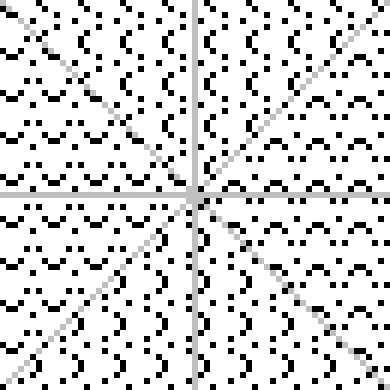
\includegraphics[scale=0.5]{rotation1} & 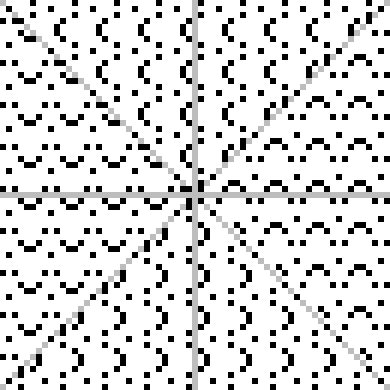
\includegraphics[scale=0.5]{rotation2} \\
		A) Actual & B) Rotation only (Incorrect)
	\end{tabular}
	\caption{In B, divisible points from quadrant 1 are rotated about the origin---no translation added, resulting in subtle differences between quadrants 2, 3, and 4 of the two plots.}
	\label{rotation}
\end{figure}

The coefficient (\(5 - 2d + k_1p\)) of the term with degree 1 changes. On the graph of any quadratic relationship, this results in a translation of the parabola. This signifies that the similarity between two quadrants relies not only on a rotation, but a translation applied afterwards. The location of a parabola can be determined by its vertex, \(A\hat{u}+B\hat{v}\). A translation of the vertex is also a translation of all divisible points on the parabola.
\begin{align}
	\nonumber \text{Original: }&\mathbf{d=D_1:}\ A_{\mathbf{D_1}}\hat{u}+B_{\mathbf{D_1}}\hat{v} \\
	\nonumber \text{Rotated: }&\mathbf{d=D_2:}\ A_{\mathbf{D_1}}\hat{u}+B_{\mathbf{D_1}}\hat{v} \\
	\nonumber \text{Actual: }&\mathbf{d=D_2:}\ A_{\mathbf{D_2}}\hat{u}+B_{\mathbf{D_2}}\hat{v}
\end{align}
	
The discrepancy between the two is the translation \(\Delta A_{D_1 \rightarrow D_2}\hat{u}+\Delta B_{D_1 \rightarrow D_2}\hat{v}\) that is needed to move the rotated vertex to its expected location.
\begin{align}
	\nonumber \Delta A_{D_1 \rightarrow D_2} &\equiv A_{D_2} - A_{D_1}\ (\text{mod }p) \\
	\nonumber \Delta B_{D_1 \rightarrow D_2} &\equiv B_{D_2} - B_{D_1}\ (\text{mod }p)
\end{align}

The translation only needs to be calculated once, then rotation symmetry can be expressed for any point:
	\[d=D_1:a\hat{u}+b\hat{v} \rightleftharpoons d=D_2:(a + \Delta A_{D_1 \rightarrow D_2})\hat{u}+(b + \Delta B_{D_1 \rightarrow D_2})\hat{v}\]
	

\subsection{Testing symmetries}

To confirm that the symmetries and their consequences are accurately understood, divisibility plots are constructed following two distinct methods. The first method uses the recursive definition of \(f\) and tests each point's divisibility. The second method finds some divisible points, and transforms those points to fill the plane. In Figure \ref{symmetryplots}, the plots are identical by visual comparison, validating the symmetries.

\begin{figure}[h!]
	\centering
	\begin{tabular}{cc}
	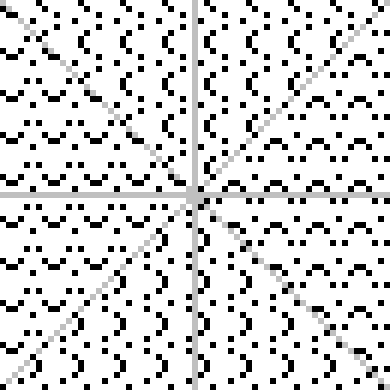
\includegraphics[scale=0.7]{m5_n4_p7_d} & 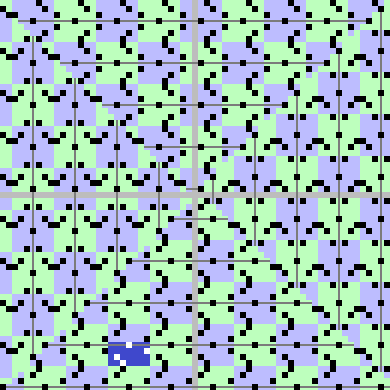
\includegraphics[scale=0.7]{m5_n4_p7_s}
	\end{tabular}
	\caption{Above, \(7 \mid f_{5,4}(P)\). Below, \(17 \mid f_{2,3}(P)\). The plots on the right are generated by the half-tiles highlighted on the plot.}
	\begin{tabular}{cc}
	& \\
	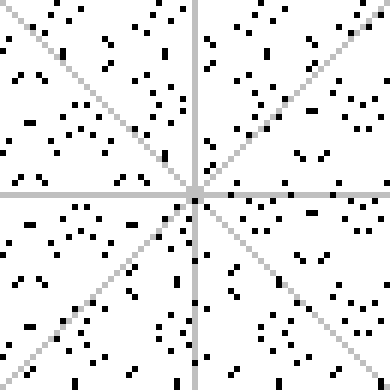
\includegraphics[scale=0.7]{m2_n3_p17_d} & 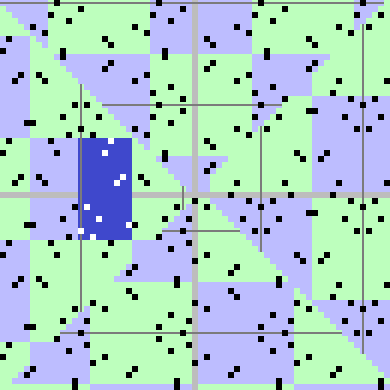
\includegraphics[scale=0.7]{m2_n3_p17_s}
	\end{tabular}
	\label{symmetryplots}
\end{figure}



\section{Lines}

Every line \(L\) on the Ulam spiral can be expressed in vector form, starting at some initial point \(a_0\hat{u}+b_0\hat{v}\), and extending along a direction vector \(\vec{\omega}=\omega_a\hat{u}+\omega_b\hat{v}\ ,\ \omega_a,\omega_b \in \mathbb{Z}\). Lines are assumed to be confined to a single quadrant.
\begin{align}
	\nonumber \mathbf{Vector\ form\ of}\ L:&d=D:(a_0\hat{u}+b_0\hat{v})+t(\omega_a\hat{u}+\omega_b\hat{v}),\ t \in \mathbb{Z} \\
	\nonumber \mathbf{Parametric\ form\ of}\ L:&d=D:\begin{cases}
										   a=a_0+t\omega_a \\
										   b=b_0+t\omega_b
										   \end{cases} = (a_0+t\omega_a)\hat{u} + (b_0+t\omega_b)\hat{v},\ t \in \mathbb{Z}
\end{align}

A ``divisible line'' modulo \(p\) contains at least one divisible point; an ``indivisible line'' contains none. Indivisible lines are desirable in the model, as they are more likely to contain prime points. \textit{Which lines are indivisible modulo \(p\)?} The question appears difficult to answer, since there are infinitely many possible lines.

When a transformation from the previous section is applied to the line \(L\), it is applied to every point in \(L\). When a divisible point is transformed, its new location is also divisible; when an indivisible point is transformed, its new location is indivisible. The transformed line \(L'\) is composed only of these transformed points. Thus, \(L'\) must have the same divisibility as \(L\). In this way, \(L\) and \(L'\) are redundant, and knowing the divisibility of \(L\) automatically grants knowledge about the divisibility of \(L'\).
	\[L \leftrightharpoons L'\]

In the following sections, symmetry is used to show how every line is redundant to a simpler line expressible in the form \(d=D:(sb+c)\hat{u}+b\hat{v}\ ,\ s,c \in \mathbb{Z}\ ,\ 0 \leq s,c < p\). One may find the divisibility of each line in the simplified form, then use symmetry to determine the divisibility of every possible line.


\subsection{Translational symmetry}

\begin{figure}[h!]
	\centering
	\begin{tabular}{cc}
		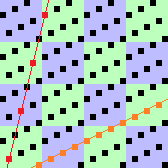
\includegraphics{trans1} & 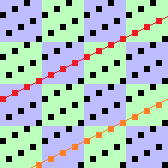
\includegraphics{trans2}
	\end{tabular}
	\caption{In each divisibility plot modulo 7, the red line is redundant to the orange line by translational symmetry.}
	\label{trans}
\end{figure}

Recall the tiling conjecture: \(P \rightleftharpoons P + k_ap\hat{u} + k_bp\hat{v}\ ,\ k_a,k_b \in \mathbb{Z}\).

\begin{align}
	\nonumber L:d=D:\begin{cases}
			a=a_0+t\omega_a \\
			b=b_0+t\omega_b
			\end{cases}
	  &\rightleftharpoons L':d=D:\begin{cases}
									 a=a_0+t\omega_a+k_ap=(a_0+k_ap)+t\omega_a \\
									 b=b_0+t\omega_b+k_bp=(b_0+k_bp)+t\omega_b
									 \end{cases} \\
	\nonumber L:d=D:\begin{cases}
			a=a_0+t\omega_a \\
			b=b_0+t\omega_b
			\end{cases}
	  &\rightleftharpoons L':d=D:\begin{cases}
									 a=a_0+t\omega_a+tk_ap=a_0+t(\omega_a+k_ap) \\
									 b=b_0+t\omega_b+tk_bp=b_0+t(\omega_b+k_bp)
									 \end{cases}
\end{align}

As shown, adding multiples of \(p\) to any of \(a_0,b_0,\omega_a,\omega_b\) results in a line redundant to the original.

\paragraph{Translational symmetry principle of lines A} If
\(a_0 \equiv a_0'\ ,\ b_0 \equiv b_0'\ ,\ \omega_a \equiv \omega_a'\ ,\ \omega_b \equiv \omega_b'\ (\text{mod }p)\), then
	\[L:d=D:\begin{cases}a=a_0+t\omega_a \\b=b_0+t\omega_b\end{cases} \rightleftharpoons L':d=D:\begin{cases}a=a_0'+t\omega_a' \\b=b_0'+t\omega_b'\end{cases}\] 

Thus, every line is redundant to some line where \(0 \leq a_0,b_0,\omega_a,\omega_b < p\). 

\paragraph{Lines where \(\omega_b \equiv 0\ (\text{mod }p)\)} make up a small portion of all lines on the plot. Ideally, these lines may be studied further, but in this essay they are assumed unnoteworthy and ignored for brevity.

\paragraph{Lines where \(\omega_b \not\equiv 0\ (\text{mod }p)\)} can be simplified by the substitution \(t = t' \omega_{b_p}^{-1}\).
	\[L:d=D:\begin{cases}
			a=a_0+t\omega_a=a_0+t' b^{-1}_p\omega_a=a_0+t'(\omega_{b_p}^{-1}\omega_a)\\
			b=b_0+t\omega_b=b_0+t' b^{-1}_p\omega_b=b_0+t'(\omega_{b_p}^{-1}\omega_b)
			\end{cases}\]

Consider \(L':d=D:\begin{cases}a=a_0+t{\omega_b^{-1}}_p\omega_a \\ b=b_0+t \end{cases}\). This line is redundant to \(L\) if:
	\[a_0 \equiv a_0\ ,\ b_0 \equiv b_0\ ,\ \omega_{b_p}^{-1}\omega_a \equiv \omega_{b_p}^{-1}\omega_a\ ,\ \omega_{b_p}^{-1}\omega_b \equiv 1\ (\text{mod }p)\]

All of these statements are true, thus every line where \(\omega_b \not\equiv 0\ (\text{mod }p)\) can be converted to a line where \(\omega_b = 1\).

When \(\omega_b = 1\ (\text{mod }p)\), the substitution \(b=b_0+t \rightarrow t=b-b_0\) can be used:
	\[L:d=D:\begin{cases}
			a=a_0+t\omega_a \rightarrow a=a_0+(b-b_0)\omega_a=(a_0-b_0\omega_a)+b\omega_a \\
			b=b_0+t \rightarrow b=b_0+(b-b_0)=b
			\end{cases}\]

Let \(s\) be the slope of the line with respect to \(\hat{v}\): \(s = \frac{\omega_a}{\omega_b} = \frac{\omega_a}{(1)} = \omega_a\). \(c\) is the \(a\)-intercept of the line (when \(b=0\)): \(c = \omega_a(0) + a_0 = a_0\). The line can be written in the form \(L:d=D:a=sb+c\).

\paragraph{Translational symmetry principle of lines B} The translational symmetry principle of lines can be adapted to lines of this form. If \(s \equiv s'\ ,\ c \equiv c'\ (\text{mod }p)\), then
	\[L:d=D:a=sb+c \rightleftharpoons L':d=D:a=s' b+c'\] 

Thus, every line is redundant to some line where \(0 \leq c,s < p\).


\subsection{Rotational symmetry}

In rotational symmetry,
	\[\Delta A_{D_1 \rightarrow D_2} = A_{D_2}-A_{D_1}\]
	\[\Delta B_{D_1 \rightarrow D_2} = B_{D_2}-B_{D_1}\] 	
	\[d=D_1:a\hat{u}+b\hat{v} \rightleftharpoons d=D_2:(b + \Delta A_{D_1 \rightarrow D_2})\hat{u}+(b + \Delta B_{D_1 \rightarrow D_2})\hat{v}\]
	
This can be applied to lines.
	\[L:d=D_1:a=sb+c \rightleftharpoons L':d=D_2:(a - \Delta A_{D_1 \rightarrow D_2})=s(b - \Delta B_{D_1 \rightarrow D_2})+c\]
	\[L':d=D_2:a=sb + (c-s\Delta B_{D_1 \rightarrow D_2}+\Delta A_{D_1 \rightarrow D_2})\]

Letting \(D_2=1\), every line is redundant to some line in quadrant 1. In conclusion, every line may be converted to the form \(d=1:a=sb+c\ ,\ 0 \leq c,s < p\). In total, there are \(p^2\) unique lines.


\subsection{Divisible lines modulo 2}

First, this special case is considered, to demonstrate the process of finding an indivisible line.

\(L:d=D:a=sb+c\) is divisible if there exists some point on \(L\) that is divisible---there is some value of \(b\) for which the point \(d=D:(sb+c)\hat{u}+b\hat{v}\) on the line is divisible. Whether \(b\) exists may be determined by attempting to construct it. Begin by assuming that \(d=D:(sb+c)\hat{u}+b_0\hat{v}\) is a divisible point.
\begin{align}
	\nonumber d=D:2 \mid f_{m,n}((sb+c)\hat{u}+b\hat{v}) \\
	\nonumber (4(sb+c)^2 - 5(sb+c) + 2D(sb+c) + b)m + n &\equiv 0\ (\text{mod }2) \\
	\nonumber bm(s + 1) + cm + n &\equiv 0\ (\text{mod }2)
\end{align}

If \(m\) is even, then \(n \equiv 0\ (\text{mod }2) \Rightarrow 2 \mid n\). This is always false (has no solution) if \(n\) is odd. When \(m\) is odd:
\begin{align}
	\nonumber b(s + 1) &\equiv c + n \mod 2 \\
	\nonumber b &\equiv \begin{cases}
			   (s + 1)^{-1}_2(c + n)	& \text{if } 2 \nmid s + 1 \Rightarrow 2 \mid s \\
			   \text{any value}			& \text{if } 2 \mid s + 1,2 \mid c + n \\
			   \text{no solution}		& \text{if } 2 \mid s + 1,2 \nmid c + n \Rightarrow 2 \nmid s, 2 \nmid c + n
	\end{cases}\ (\text{mod }2)
\end{align}

Therefore, \(L\) is indivisible if \(m\) is even but \(n\) is odd, or if \(s\) and \(c + n\) are odd.


\subsection{Divisibility of a line}

Just as in the previous section, to determine if \(L:d=1:a=sb+c\) is divisible, begin by assuming that \(d=1:(sb+c)\hat{u}+b\hat{v}\) is a divisible point.
\begin{align}
	d=1:f_{m,n}((sb+c)\hat{u}+b\hat{v}) &\equiv 0\ (\text{mod }p) \\
	(4(sb+c)^2 - 5(sb+c) + 2(1)(sb+c) + b)m + n &\equiv 0\ (\text{mod }p) \\
	4s^2b^2 + (8sc - 3s + 1)b + 4c^2 - 3c + m^{-1}_pn &\equiv 0\ (\text{mod }p)
\end{align}
	
Let \(4s^2 = \alpha\), \(8sc - 3s + 1 = \beta\), and \(4c^2 - 3c + m^{-1}_pn = \gamma\). \(\alpha,\beta,\gamma \in \mathbb{Z}\).
\begin{align}
	\nonumber \alpha b^2 + \beta b + \gamma b &\equiv 0\ (\text{mod }p) \\
	\nonumber 4 \alpha^2 b^2 + 4 \alpha \beta b + 4 \alpha \gamma &\equiv 0\ (\text{mod }p) \\
	\nonumber (2 \alpha b + \beta)^2 - \beta^2 + 4 \alpha \gamma &\equiv 0\ (\text{mod }p) \\
	\nonumber (2 \alpha b + \beta)^2 &\equiv \beta^2 - 4 \alpha \gamma\ (\text{mod }p)
\end{align}

If \(\beta^2 - 4 \alpha \gamma\) is a quadratic nonresidue modulo \(p\), then there is no value of \(r\) that can satisfy \(r^2 \equiv \beta^2 - 4 \alpha \gamma\ (\text{mod }p)\). Thus, there is no solution for \(2 \alpha b + \beta\), and no value of \(b\) for which the assumption ``\(d=1:(sb+c)\hat{u}+b\hat{v}\) is a divisible point'' is true. In this case, \(L\) is indivisible.

To manipulate \(\beta^2 - 4 \alpha \gamma\) so that it is a quadratic nonresidue, quadratic nonresidues modulo \(p\) must first be found. This is done quickly through brute force. Numbers from \(0\) to \(p-1\) are listed. Every number that is congruent to a perfect square modulo \(p\) is a quadratic residue, and is removed. The \(\frac{p-1}{2}\) values that remain in the list are quadratic nonresidues modulo \(p\). Next, for each value \(q\) from the list, one considers the congruence:
\begin{align}
	\nonumber q &\equiv \beta^2 - 4 \alpha \gamma\ (\text{mod }p) \\
	\nonumber q &\equiv (8sc - 3s + 1)^2 - 4 (4s^2) (4c^2 - 3c + m^{-1}_pn)\ (\text{mod }p) \\
	\nonumber q &\equiv (64s^2c^2 - 48s^2c + 16sc + 9s^2 - 6s + 1) - (64s^2c^2 - 48s^2c + 16s^2m^{-1}_pn)\ (\text{mod }p) \\
	\nonumber q &\equiv 9s^2 - 16s^2m^{-1}_pn + 16sc - 6s + 1\ (\text{mod }p) \\
	\nonumber -16sc &\equiv 9s^2 - 16s^2m^{-1}_pn - 6s + 1 - q\ (\text{mod }p) \\
	\nonumber c &\equiv -16^{-1}_p9s + sm^{-1}_pn + 8^{-1}_p3 + (q-1)16^{-1}_ps^{-1}_p\ (\text{mod }p)
\end{align}
	
This suggests that there are many ways to manipulate a line so that it is indivisible. For every value of \(s\) except \(s \equiv 0\ (\text{mod }p)\), there is a possible solution for \(c\). In translational symmetry, it is shown that only \(0 \leq s < p\) needs to be studied to know the divisibility of every line. Thus, \(s\) may be varied from \(1\) to \(p-1\), evaluating \(c\) in each case. This is a finite process, involving \(\frac{p-1}{2}\) possible values for \(q\), and \(p-1\) possible values for \(p\), a total of \(\frac{(p-1)^2}{2}\) times the congruence needs to be evaluated to determine every indivisible line in the divisibility plot modulo \(p\).

\begin{figure}[h!]
	\centering
	\begin{tabular}{m{0.6\textwidth}m{0.3\textwidth}}
		\centering
		\(c \equiv -16^{-1}_79s + s(2)^{-1}_7(1) + 8^{-1}_73 + ((3)-1)16^{-1}_7s^{-1}_7\ (\text{mod }7)\)
		\[c \equiv -(4)9s + s(4)(1) + (1)3 + (2)(4)s^{-1}_7 \equiv 3s + 3 + s^{-1}_7\ (\text{mod }7)\]
		\begin{tabular}{|c|c|c|}
			\hline
			Colour & \(s\) & \(c\) \\
			\hline
			red & 1 & 0 \\
			orange & 2 & 6 \\
			yellow & 3 & 3 \\
			green & 4 & 3 \\
			blue & 5 & 0 \\
			violet & 6 & 6 \\
			\hline
		\end{tabular} &
		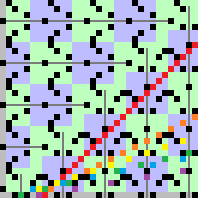
\includegraphics{rainbow}
	\end{tabular}
	\caption{When searching for indivisible lines on the divisibility plot of \(f_{2,1}\) modulo 7, it is found that 3 is a quadratic nonresidue modulo 7. Each resulting indivisible line \(d=1:a=sb+c\) is shown.}
	\label{rainbow}
\end{figure}



\section{Finding prime-rich lines}

After the procedure in section 5, the model possesses a vast collection of statements: \(L:d=1:a=sb+c\) is indivisible modulo \(p\). This can be expressed by the notation \(L:d=1:a=sb+c\ (p)\).

Statements can be combined. Choose \(k\) statements, each about a different divisibility plot:
	\[L_1:d=1:a=s_1b+c_1\ (p_1)\]
	\[L_2:d=1:a=s_2b+c_2\ (p_2)\]
	\[\cdots\]
	\[L_k:d=1:a=s_kb+c_k\ (p_k)\]
	
The goal of processing this information is to find a line \(L'\) that is redundant to every line presented in the statements. \(L'\) would be indivisible modulo every prime from \(p_1\) to \(p_k\). As explained in section 2, \(L'\) would be prime-rich. Successfully predicting its existence answers the research question affirmatively. Specifically,
	\[Q=\frac{p_1}{p_1-1}\times\frac{p_2}{p_2-1}\times\ldots\times\frac{p_k}{p_k-1}=\prod_{i=1}^k\frac{p_i}{p_i-1}\]
	
\begin{enumerate}
	\item As with every line, the target line \(L'\) is expressible in the form \(L':d=D:(a_0'+t\omega_a')\hat{u}+(b_0'+t\omega_b')\hat{v}\).
	\item Suppose one wishes to find \(L'\) in quadrant \(D\). Every statement \(L_k:d=1:a=s_kb+c_k\ (p_k)\) is converted into \(L_k:d=D:a=s_kb+(c_k-s_k\Delta B_{1 \rightarrow D}+\Delta A_{1 \rightarrow D})\ (p_k)\), following rotational symmetry.
	\item The line \(L_k:d=D:a=s_kb+c_k\) can be converted into a vector form, by reversing the substitutions described in section 5.1. In this way, every statement returns to one in the form
		\[L_k:d=D:(a_{0_k}+t\omega_{a_k})\hat{u}+(b_{0_k}+t\omega_{b_k})\hat{v}\ (p_k)\]
	\item From the translational symmetry principle of lines, it is known that \(L'\) is redundant to \(L_k\) if
		\[a_{0_k} \equiv a_0'\ ,\ b_{0_k} \equiv b_0'\ ,\ \omega_{a_k} \equiv \omega_a'\ ,\ \omega_{b_k} \equiv \omega_b'\ (\text{mod }p_k)\]
	Therefore,
	\begin{align}
		\nonumber a_{0_1} &\equiv a_0'\ (\text{mod }p_1) \\
		\nonumber a_{0_2} &\equiv a_0'\ (\text{mod }p_2) \\
		\nonumber &\cdots \\
		\nonumber a_{0_k} &\equiv a_0'\ (\text{mod }p_k)
	\end{align}
	And similarly for \(b_0,\omega_a,\omega_b\).
	\item For each of \(a_0',b_0',\omega_a',\omega_b'\), the system of congruences may be solved by implementing the Chinese remainder theorem. In fact, a solution must exist, therefore the statements may always be combined to find \(L'\).
\end{enumerate}

Thus, in the model, arbitrarily many statements can be combined to predict the location of a line that is indivisible by an arbitrary number of primes. Considering the number of statements available for each \(p\), the number of solutions to \(L'\) is so vast that it would be impractical to use a model that finds them all.


\subsection{Algorithm}

The model generates a random solution for \(L'\) in the plot of \(f_{m,n}\) which does not contain multiples of the first \(k\) primes.

\begin{enumerate}
	\item Generate a list of the first \(k\) primes. For each prime \(p_i\):
	\item If \(p_i \mid m\), then if \(p_i \mid n\), the plot will contain no prime-rich lines, and the algorithm may abort. If \(p_i \nmid n\), the algorithm may continue, and this value of \(p_i\) may be skipped, since the plot of \(f_{m,n}\) contains no divisible points modulo \(p_i\).
	\item For \(D = 2,3,4\), \(\Delta A_{1 \rightarrow D}\) and \(\Delta B_{1 \rightarrow D}\) are calculated.
	\item The guess-and-check method determines all quadratic nonresidues \(q\) modulo \(p_i\).
	\item For each possible \(q\), for each value \(s\) from \(1\) to \(p-1\), \(c \equiv -16^{-1}_{p_i}9s + sm^{-1}_{p_i}n + 8^{-1}_{p_i}3 + (q - 1)16^{-1}_{p_i}s^{-1}_{p_i}\ (\text{mod }p_i)\) is evaluated and stored in a list of statements about \(p_i\).
	\item One statement is selected randomly from the list of statements about \(p_i\).
	\item \(D\) is selected at random, and all statements are converted accordingly.
	\item For each statement, \(b_0\) is chosen between 0 and \(p_i-1\), and \(\omega_b\) is chosen between 1 and \(p_i-1\). \(d=D:a=sb+c\) is rewritten as \(d=D:\begin{cases}a=st'+c \\ b=t'\end{cases}\), where \(t' = b_0 + t\omega_b\). Then \(a = s(b_0 + \omega_bt)+c = sb_0 + s\omega_bt + c\), thus \(a_0 = sb_0 + c\) and \(\omega_a = s\omega_b\).
	\item The Chinese remainder theorem is used to solve for \(a_0',b_0',\omega_a',\omega_b'\).
\end{enumerate}


\subsection{Results}

\begin{figure}[h!]
	\resizebox{\textwidth}{!}{%
	\begin{tabular}{|c|c|c|}
		\hline
		\(k = 3\) & \(k = 4\) & \(k = 5\) \\
		\(Q = 3.75\) & \(Q = 4.375\) & \(Q = 4.8125\) \\
		\hline
		\(d = 3: (0 + 23t)\hat{u} + (-14 + -7t)\hat{v}\) & \(d = 1: (183 + 11t)\hat{u} + (49 + 101t)\hat{v}\) & \(d = 3: (487 + 851t)\hat{u} + (1109 + -293t)\hat{v}\) \\
		\(d = 3: (28 + 23t)\hat{u} + (14 + -7t)\hat{v}\) & 	\(d = 4: (119 + 71t)\hat{u} + (-3 + 89t)\hat{v}\) & 
		\(d = 3: (2172 + 61t)\hat{u} + (-540 + -61t)\hat{v}\) \\
		\(d = 2: (19 + 29t)\hat{u} + (1 + -7t)\hat{v}\) & 
		\(d = 1: (115 + 131t)\hat{u} + (87 + -11t)\hat{v}\) & 
		\(d = 3: (1549 + 13t)\hat{u} + (155 + -377t)\hat{v}\) \\
		\(d = 2: (5 + 17t)\hat{u} + (11 + 17t)\hat{v}\) & 
		\(d = 1: (37 + 167t)\hat{u} + (-33 + -59t)\hat{v}\) & 
		\(d = 3: (579 + -989t)\hat{u} + (609 + -1873t)\hat{v}\) \\
		\(d = 4: (1 + 19t)\hat{u} + (3 + -1t)\hat{v}\)
& 
		\(d = 3: (36 + 107t)\hat{u} + (-102 + -101t)\hat{v}\)
& 
		\(d = 2: (345 + 353t)\hat{u} + (627 + 821t)\hat{v}\) \\
		\hline
	\end{tabular}}
	\caption{These theoretically prime-rich lines in the plots of \(f_{1,1}\) were produced near instantaneously by the computer.}
	\resizebox{\textwidth}{!}{
	\begin{tabular}{|c|c|}
		\hline
		\(k = 6\) & \(k = 7\) \\
		\(Q = 5.213541\bar{6}\) & \(Q = 5.5393880208\bar{3}\) \\
		\hline
		\(d = 4: (4190 + -13781t)\hat{u} + (11282 + -29647t)\hat{v}\) & \(d = 1: (87308 + -64321t)\hat{u} + (-70090 + -275453t)\hat{v}\) \\
		\(d = 4: (26505 + 9241t)\hat{u} + (-13949 + -11191t)\hat{v}\) & \(d = 4: (371753 + -455761t)\hat{u} + (203541 + -510481t)\hat{v}\) \\
		\(d = 4: (14181 + -14813t)\hat{u} + (1285 + -26977t)\hat{v}\) & \(d = 2: (418792 + 212521t)\hat{u} + (175024 + -56471t)\hat{v}\) \\
		\(d = 1: (2055 + 193t)\hat{u} + (-3359 + 4423t)\hat{v}\) & \(d = 3: (200891 + -262517t)\hat{u} + (229281 + -307253t)\hat{v}\) \\
		\(d = 4: (27360 + 22531t)\hat{u} + (-13520 + -12541t)\hat{v}\)
& \(d = 4: (133831 + -321137t)\hat{u} + (-104149 + -400481t)\hat{v}\) \\
		\hline
	\end{tabular}}
	\label{outputs}
\end{figure}

\(a_0',b_0',\omega_a',\omega_b'\) grow rapidly in magnitude with \(k\), while \(Q\) grows slowly. For \(k > 8\), the values of \(f\) for points along the lines produced are in the quadrillions. This is the greatest disadvantage of this model.
\begin{align}
\nonumber f_{m,n}(a\hat{u}+b\hat{v}) &= (4a^2 - 5a + 2da + b)m + n \equiv 0 \mod p \\
\nonumber f_{m,n}(a\hat{u}+b\hat{v}) &\approx 4ma^2 \\
\nonumber f_{m,n}((a_0'+t\omega_a')\hat{u}+(b_0'+t\omega_b')\hat{v}) &\approx 4m(a_0'+t\omega_a')^2 \\
\nonumber P(X \in \mathbb{P}|X \approx f_{m,n}((a_0'+t\omega_a')\hat{u}+(b_0'+t\omega_b')\hat{v})) &\approx P(X \in \mathbb{P}|X \approx 4m(a_0'+t\omega_a')^2)
\end{align}
	
This is approximately \(\frac{1}{\ln(4m(a_0+t\omega_a')^2) - 1.08366}\). When \(a_0'\) or \(\omega_a\) are large, the probability that \(X\) is prime is small despite a large \(Q\), and the model still fails to produce an abundance of prime numbers.

This is avoided somewhat by altering steps 2a and 2c. In 2a, one chooses statements where \(s = 1\). In 2c, one chooses \(\omega_b = 1\). Thus, \(\omega_a' \equiv 1\ (\text{mod }p_i)\), to which \(\omega_a' = 1\) is always a solution.


\subsection{Evaluation}

250 lines are produced by the simplied model. On each line, the number of prime points first 250 points with the least a value is recorded. This is repeated without the model, checking 250 lines generated randomly.

\(R\) is the actual ratio of primes found by the model divided by primes found without the model. \(R\) varies somewhat from its expected values, however its general trend matches \(Q\).

\begin{figure}[h!]
	\centering
	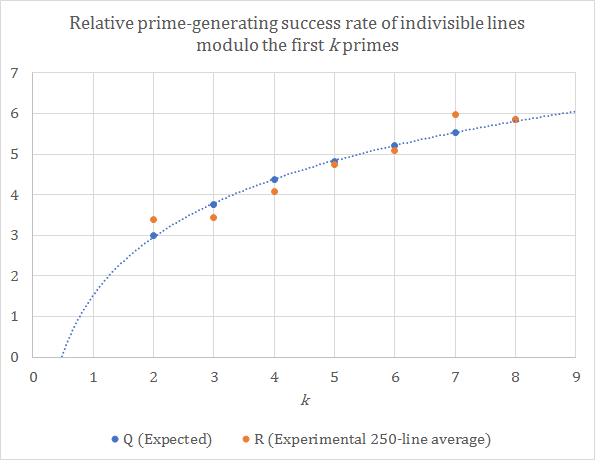
\includegraphics{graph}
	\caption{The above graph uses information gathered from \(f_{1,1}\). All lines considered were in the form \((a_0\hat{u}+b_0\hat{v})+t(\hat{u}+\hat{v})\).}
	\label{graph}
\end{figure}

	
	
\section{Conclusion}

Mathematically, it was discussed how a model may locate every possible line indivisible by arbitrarily many primes, on any spiral. The lines that have been checked yield primes at about the same rate as the model predicts. The model can achieve a fivefold increase in the probability of generating a prime number. This is not particularly large. However, it is sufficient to show that the Ulam spiral's ``mystery'' has yet another valid explanation. The significance of a structure perceived in imperfect randomness is usually the existence of more underlying structures.



\newpage

\begin{thebibliography}{1}
	
\bibitem{}
Bates, T. (n.d.). Ulam Spiral. \\
Retrieved February 05, 2018, from \\ 			
\url{http://www.betweenartandscience.com/ulamspiral_words.html}
	
\bibitem{}
Granville, A. (n.d.). Harald Cramér and the Distribution of Prime Numbers. \\
Retrieved February 5, 2018, from \\ 
\url{https://www.dartmouth.edu/~chance/chance_news/for_chance_news/Riemann/cramer.pdf} \\
Athens, Georgia, USA.

\bibitem{}
Inglis-Arkell, E. (2011, July 09). The Bizarre Mathematical Conundrum Of Ulam's Spiral. \\ Retrieved February 05, 2018, from \\ \url{https://www.gizmodo.com.au/2011/07/the-bizarre-mathematical-conundrum-of-ulams-spiral/}

\bibitem{}
Ribenboim, P. (2004). The little book of bigger primes (2nd ed.). New York: Springer. \\
Accessed February 5, 2018

\bibitem{}
Sacks, R. (n.d.). NumberSpiral.com. \\
Retrieved February 05, 2018, from \\
\url{https://www.numberspiral.com/index.html}

\bibitem{}
Stein, M. L., Ulam, S. M., \& Wells, M. B. (1964). A Visual Display of Some Properties of the Distribution of Primes. The American Mathematical Monthly, 71(5), 516-520. doi:10.2307/2312588

\bibitem{}
Wright, S. (2016). \textit{Quadratic residues and non-residues: selected topics.} Switzerland: Springer. \\
Accessed February 5, 2018
	
\end{thebibliography}


\newpage
\appendix

\section{Indivisible lines modulo primes up to 17}

For any of the listed primes \(p\), any quadratic nonresidue \(r\) may be chosen from the respective table to give a value of \(c\) for which \(d=1:a=sb+c\) is an indivisible line modulo \(p\) on the divisibility plot of \(f_{1,1}\). Symmetries can then be used to find all other indivisible lines.

\begin{center}
	
\[p = 3\]
\begin{tabular}{cc|c|c|}
	&              & \multicolumn{2}{c|}{\textbf{s}} \\
	& \textbf{c}   & 1& 2 \\ \hline
	\textbf{r} & 2 & 2& 1 \\ \hline
\end{tabular}
\bigskip

\[p = 5\]
\begin{tabular}{cc|c|c|c|c|}
	&                               & \multicolumn{4}{c|}{\textbf{s}} \\
	& \textbf{c}                    & 1& 2& 3& 4 \\ \hline
	\multirow{2}{*}{\textbf{r}} & 2 & 4& 3& 4& 3 \\ \cline{2-6}
	                            & 3 & 0& 1& 1& 2 \\ \hline
\end{tabular}
\bigskip

\[p = 7\]
\begin{tabular}{cc|c|c|c|c|c|c|}
	&                               & \multicolumn{6}{c|}{\textbf{s}} \\
	& \textbf{c}                    & 1& 2& 3& 4& 5& 6 \\ \hline
	\multirow{3}{*}{\textbf{r}} & 3 & 4& 0& 1& 5& 6& 2 \\ \cline{2-8}
	                            & 5 & 5& 4& 6& 0& 2& 1 \\ \cline{2-8}
	                            & 6 & 2& 6& 5& 1& 0& 4 \\ \hline
\end{tabular}
\bigskip

\[p = 11\]
\begin{tabular}{cc|c|c|c|c|c|c|c|c|c|c|}
	&                               & \multicolumn{10}{c|}{\textbf{s}} \\
	& \textbf{c}                    & 1& 2& 3& 4& 5& 6& 7& 8& 9&10 \\ \hline
	\multirow{5}{*}{\textbf{r}} & 2 & 5& 3& 4& 3&10&10& 6& 5& 6& 4 \\ \cline{2-12}
								& 6 & 8&10& 5& 1& 4& 5& 8& 4&10& 1 \\ \cline{2-12}
								& 7 & 6& 9& 8& 6& 8& 1& 3& 1& 0& 3 \\ \cline{2-12}
								& 8 & 4& 8& 0& 0& 1& 8& 9& 9& 1& 5 \\ \cline{2-12}
								&10 & 0& 6& 6&10& 9& 0&10& 3& 3& 9 \\ \hline
\end{tabular}
\bigskip

\[p = 13\]
\begin{tabular}{cc|c|c|c|c|c|c|c|c|c|c|c|c|}
&                               & \multicolumn{12}{c|}{\textbf{s}} \\
& \textbf{c}                    & 1& 2& 3& 4& 5& 6& 7& 8& 9&10&11&12 \\ \hline
\multirow{6}{*}{\textbf{r}} & 2 & 9& 9&12& 6&12&11& 6& 5&11& 5& 8& 8 \\ \cline{2-14}
							& 5 &10& 3& 8& 3& 7& 9& 8&10& 1& 9& 1& 7 \\ \cline{2-14}
							& 6 & 6& 1&11& 2& 1& 4& 0& 3& 2& 6& 3&11 \\ \cline{2-14}
							& 7 & 2&12& 1& 1& 8&12& 5& 9& 3& 3& 5& 2 \\ \cline{2-14}
							& 8 &11&10& 4& 0& 2& 7&10& 2& 4& 0& 7& 6 \\ \cline{2-14}
							&11 &12& 4& 0&10&10& 5&12& 7& 7& 4& 0& 5 \\ \hline
\end{tabular}
\newpage

\[p = 17\]
\begin{tabular}{cc|c|c|c|c|c|c|c|c|c|c|c|c|c|c|c|c|}
	&                               & \multicolumn{16}{c|}{\textbf{s}} \\
	& \textbf{c}                    & 1& 2& 3& 4& 5& 6& 7& 8& 9&10&11&12&13&14&15&16 \\ \hline
	\multirow{8}{*}{\textbf{r}} & 3 & 2&13&12& 8&13&14& 3&10&12& 2& 8& 9&14&10& 9& 3 \\ \cline{2-18}
								& 5 & 0&12& 0&16&16& 8&10&14& 8&12&14& 6& 6& 5&10& 5 \\ \cline{2-18}
								& 6 &16& 3&11& 3& 9& 5& 5&16& 6& 0& 0&13& 2&11& 2& 6 \\ \cline{2-18}
								& 7 &15&11& 5& 7& 2& 2& 0& 1& 4& 5& 3& 3&15& 0&11& 7 \\ \cline{2-18}
								&10 &12& 1& 4& 2&15&10& 2& 7&15& 3&12& 7& 3& 1& 4&10 \\ \cline{2-18}
								&11 &11& 9&15& 6& 8& 7&14& 9&13& 8&15&14&16& 7&13&11 \\ \cline{2-18}
								&12 &10& 0& 9&10& 1& 4& 9&11&11&13& 1& 4&12&13& 5&12 \\ \cline{2-18}
								&14 & 8&16&14& 1& 4&15&16&15& 7& 6& 7& 1& 4& 8& 6&14 \\ \hline
\end{tabular}
\bigskip
	
\end{center}



\section{Model test data}

\centering
\begin{tabular}{|c|c|c|c|c|c|c|c|}
	\hline
	\(k\)	&2	&3	&4	&5	&6	&7	&8 \\
	\hline
	\(Q\)	&3	&3.75	&4.37\ldots	&4.81\ldots	&5.21\ldots	&5.53\ldots	&5.84\ldots \\
	\hline
	Primes found with model	&20211	&20356	&23416	&19384	&16036	&13486	&11442 \\
	\hline
	Primes found without model	&5955	&5913	&5749	&4093	&3153	&2253	&1954 \\
	\hline
	\(R\)	&3.39\ldots	&3.44\ldots	&4.07\ldots	&4.73\ldots	&5.08\ldots	&5.98\ldots	&5.85\ldots \\
	\hline
\end{tabular}



\end{document}